\documentclass[10.5,a4paper,titlepage, dvipdfmx]{bxjsarticle}
%\usepackage{zxjatype}
%\usepackage[ipa]{zxjafont}
\usepackage{comment}
\usepackage[dvipdfmx]{graphicx}
\usepackage[dvipdfmx]{color}
\usepackage{url}
\usepackage{here}
%目次にリンクをつける
%\usepackage{hyperref}
\usepackage[margin=5pt]{subcaption}
\usepackage{ascmac}
\usepackage{latexsym}
\usepackage{amsmath}
\usepackage{amssymb}
\usepackage{amsfonts}
%\usepackage{color}
\usepackage{slashbox}
\usepackage{diagbox}
%行間を開ける
\usepackage{setspace}
%定理

\usepackage[long]{optidef}

\def\qed{\hfill $\Box$}

\title{重み付きクラスター編集問題に対する効率的なアルゴリズム}
\author{木村 陸}
\date{\today}

\begin{document}
\begin{center}
    \Large 中央大学大学院理工学研究科情報工学専攻\\*修士論文 \par
    \vspace{30mm}
    \huge クラスター編集問題に対する\\*効率的な解法の研究 \par
    \vspace{15mm}
    \Large Study on Efficient Algorithms for Cluster Editing Problem \par
    \vspace{30mm}
    \Large 木村 \ 陸 \par
    \Large Riku \ Kimura \par
    \Large 学籍番号 \ 20N8100005L\par
    \vspace{15mm}
    \Large 指導教員 \quad 福永 \ 拓郎 \ 教授 \par
    \vspace{30mm}
    \Large 2022年3月
    \vspace{20mm}
\end{center}
\thispagestyle{empty}
\clearpage
\addtocounter{page}{-1}
\pagenumbering{roman}
\noindent
\begin{center}
    \Large \textbf{概要}
\end{center}\par
クラスター編集問題(または相関クラスタリング問題)は以下のように定義される最適化問題である.
無向グラフ$G$が与えられる.
各連結成分がクリークであるグラフのことをクラスターグラフと呼ぶ.
$G$に辺を追加したり, $G$から辺を削除することで$G$をクラスターグラフに変えたい.
この際に, 必要な追加$\cdot$削除の回数を最小化せよという問題である.
クラスター編集問題はタンパク質や遺伝子などのデータのクラスタリングに応用される.
したがって, クラスタリングへの応用を考えると, クラスター編集問題の大規模な問題例を現実的な時間で解く必要性が高い.
しかし, この問題はNP困難であるので, 大規模な問題に対しては厳密アルゴリズムでの計算時間は非常に大きくなってしまう.
そこで, 本研究ではより大規模な問題を厳密に解くアルゴリズムの研究を行う.
基礎的な分枝限定アルゴリズムに前処理による問題サイズの削減, 最適値の上界の計算, 再帰の深さに応じた計算の省略といった工夫を導入して計算の高速化を図る.
これらのアルゴリズムをプログラムとして実装し, 計算実験を通してその効果を検証する.\\

\noindent
\textbf{キーワード}: クラスター編集問題, クラスタリング, 分枝限定法
\clearpage

\tableofcontents
\clearpage
%行間開け
%\b2.0}egin{spacing}{
\section{はじめに}
\setcounter{page}{1}
\pagenumbering{arabic}
\textbf{クラスター編集問題}(または相関クラスタリング問題)は以下のように定義される最適化問題である.
無向グラフ$G$が与えられる.
各連結成分がクリークであるグラフのことを\textbf{クラスターグラフ}と呼ぶ.
$G$に辺を追加したり, $G$から辺を削除することで$G$をクラスターグラフに変えたい.
この際に, 必要な追加$\cdot$削除の回数を最小化せよという問題である.\par
クラスター編集問題はオブジェクトのクラスタリングへの応用を動機として導入された.
クラスタリングとは, 与えられたオブジェクト同士を互いによく似たオブジェクトによって構成される部分集合に分割するタスクのことである.
クラスター編集問題をクラスタリングに応用する際には, 頂点をオブジェクトに対応させ, 似ているオブジェクトに対応する2頂点間に辺を定義することで無向グラフを作成する.
このグラフ上でクラスター編集問題を解くことでクラスタリングを行う.
この手法は遺伝子やタンパク質をクラスタリングする際に用いられてきた[2,21,30].
他のクラスタリング手法と比べてクラスター編集問題が優れている点は, クラスターの数や各クラスターのサイズを指定する必要がない点にある.
これらの良いパラメータを選択することは, 入力データと現実世界の問題の両方に強い依存性があるためしばしば困難である.
その点クラスター編集問題は問題を解くことで自動的にクラスターの個数やサイズを決定することができる.\par
また, 一対のオブジェクトの類似性を決定することは容易だが, 3つ以上のオブジェクト全体に対して類似性を決定することは困難なことが多い.
クラスター編集問題は決定が容易なオブジェクト対の類似性から全体のクラスタリングを計算することから, 有用性も高い.
この問題はパラメータ化アルゴリズムに関するコンペティションであるPACE Challengeの2021年の課題[26]として取り上げられたことからもこの問題の重要性が伺える.\par
クラスター編集問題はNP困難であることがKřivánekとMoráve[23]により示された.
さらにAPX困難であることもCharikarら[10]によって示された.
しかしながら, クラスタリングへの応用を考えると, クラスター編集問題の大規模な問題例を現実的な時間で解く必要性が高い.
このため, CLICK[30], CAST[2], HCS[21]のようなヒューリスティックに基づくソルバーの開発も盛んである.
ただし, これらは問題の最適解を計算するわけではない.
最適解を計算する試みとしては, クラスター編集問題を整数計画問題として定式化して整数計画ソルバーを利用して解くアプローチについて研究されている[19].
しかし, このアプローチであっても実用性の面では十分ではない.\par
そこで, 本研究ではより大規模な問題を厳密に解くアルゴリズムの研究を行う.
基礎的な分枝限定アルゴリズムを実装し, そこに様々な工夫を導入する.
例えば, 前処理による問題サイズの削減, 最適解の目的関数値の上界の計算, 再帰の深さに応じた計算の省略といった工夫である.
これらのアルゴリズムをプログラムとして実装し, 計算実験を通してその効果を検証する.\par
本論文の構成は次のとおりである.
2章で先行研究を紹介する.
3章で問題設定.
4章で分枝限定アルゴリズムの戦略に必要な辺操作の説明.
5章で提案アルゴリズムの全体像.
6章で実験.
7章で結論となっている.

\section{先行研究}
\subsection{計算複雑性}
クラスター編集問題はNP困難であり, その証明は独立して発表されている[1,12,29].
初めての証明は1986年にKřivánekとMorávekら[23]によってなされた.
特に, 最大次数6のグラフでもNP困難であることが知られている[13].
また, 指数時間仮説[23]のもとでは, 頂点数$n$における準指数時間アルゴリズムは存在しない[16,24].\par

クラスター編集問題は特定のグラフに対して多項式時間で解くことができる.
例えば単位区間グラフ,最大次数2のグラフ,道, 閉路で多項式時間で解くことができる[25].
しかし, 最大次数が3から5のグラフではNP困難か多項式時間で解けるかは未解決の問題である.
クラスターグラフから「それほど遠くない」グラフに関しては, 貪欲型ヒューリスティックで多項式時間で最適解を見つけることができる[28].\par
クラスター編集問題の近似性について, Charikarら[10]はこの問題がAPX困難(1より大きいある定数倍以内で近似することがNP困難)であることを示した.


\subsection{パラメータ化アルゴリズムとデータ削減}
入力でサイズ$n$とパラメータ$k$が与えられる問題に対して, 計算量がある計算可能な関数$f$と多項式$poly$を用いて$O(f(k) \cdot poly(n))$と表せるアルゴリズムが存在するならば, その問題は固定パラメータ容易であるという[13].
クラスター編集問題は固定パラメータ容易であり, カーネルと探索木両方のアプローチによるアルゴリズムが存在する(5章参照).
最適解の目的関数値をパラメータとして使用する, パラメータ化アルゴリズムは特によく研究されている.
このパラメータ化アルゴリズムでは, 最適解の目的関数値が与えられたパラメータ$k$以下の場合, 最適解を出力する.
それ以外の場合は「解なし」というメッセージを出力する.
最適解を見つけたいが$k$がわからない場合は$k=0,1,2...$のアルゴリズムを繰り返し呼び出すことで求めることができる.\par
クラスター編集問題のパラメータ化アルゴリズムに関する最初の結果は, Grammら[18]によって与えられた.
実行時間$O(3^k+n^3)$の単純なアルゴリズムを提案し, さらにこれを洗練した分枝戦略を用いて$O(2.27^k+n^3)$へと改善した.
後にGrammら[17]は自動化された広範なケース分析によってこれを$O(1.92^k+n^3)$に改善した.
しかし, 結果として得られるアルゴリズムには, 100を超える初期分枝ケースがあり, 現在まで知る限り実装されたことはない.
クラスター編集問題にコスト関数を導入して問題を拡張することにより, 実行時間はBöckerら[3]によって$O(1.82^k+n^3)$に改善された.
その後, BöckerとDamaschkeは, 多くの衝突を含まないグラフと特性を使用して, 実行時間$O(1.76^k+m+n)$のアルゴリズムを導出した[4].
現在最速のアルゴリズムは, 特定の性質をもつグラフに限るが$O(1.62^k+m+n)$時間である[6].\par
カーネル化は, パラメータ$k$を持つ問題例$I$をパラメータ$k' \le k$を持つ新しい問題例$I'$に変換する多項式時間アルゴリズムであり, 以下の条件を満たす.
$(i)$問題例$(I,k)$は問題例$(I',k')$が解をもつ場合に限り解を持つ.
$(ii)$問題例$I'$のサイズが計算可能な関数$f$に対して最大で$f(k)$である.
カーネル化は多くの場合, 処理しやすい問題例の部分を切り取る一連の削減ルールを適用することによって実現される.
カーネルサイズ$f(k)$はカーネルの有効性の尺度を表す.\par
Grammら[18]は$O(n^3)$時間で$O(k^2)$頂点を使用したクラスター編集問題のカーネルを計算する方法を示した.
また, より高速なカーネル化は, $O(n+m)$時間で$2k^2+k$頂点を持つカーネルを計算したProttietら[27]によって与えられた.
IWPEC 2006では, Fellows[14]は, 問題の線形計画法の定式化に基づいて, $24k$の頂点を持つ多項式時間カーネルを提案した.
2007年には, Fellowら[15]は, クラウンタイプの削減に基づいて$6k$の頂点を持つ組み合わせカーネルを提案した.
Guo[20]はクリティカルクリークの概念に基づいて, $O(n^3)$時間で計算できる$4k$の頂点を持つカーネルを提示した.
これは後にChenとCao[11]によって$2k$頂点に改善された.
同様に, $O(k^2)$頂点[3]を持つ整数重みの問題のカーネルは$2k$頂点[9]に改善された.\par
カーネル法は, データ削減と見なすことできる.
パラメータ化されたデータ削減ルールは, [5]で説明されているようにパラメータに依存しないようにすることができる.
これにより, (多項式時間の)データ削減を事前に適用し, 厳密アルゴリズムあるいはヒューリスティックアルゴリズムを用いて残りの問題を解くことができる.


\section{問題設定}
本章ではクラスター編集問題の正確な問題設定を説明する.
クラスター編集問題には, コストなしクラスター編集問題とコストありクラスター編集問題の2種類がある.
3.1章でコストなしクラスター編集問題を導入し, 3.2章でコストありクラスター編集問題を導入する.

\subsection{コストなしクラスター編集問題}
$G=(V,E)$を頂点集合$V$, 辺集合$E$からなる無向グラフとする. 頂点の部分集合$C \subseteq V$に属する任意の2頂点間に辺が存在するとき, $C$から誘導される部分グラフを$G$の$\textbf{クリーク}$と言う.
グラフ内の連結成分が全てクリークであるグラフを$\textbf{クラスターグラフ}$と呼ぶ.
グラフに新たな辺を追加したり, グラフ内の辺を削除することを辺操作と呼ぶ.
コストなしクラスター編集問題とは与えられたグラフに対して辺操作を繰り返し行い, クラスターグラフに変換する問題である.\par
正確には, コストなしクラスター編集問題の問題設定は以下のように書ける.\\

\begin{screen}
    $\textbf{コストなしクラスター編集問題}$ \\
    入力: \\
    \hspace{15pt} 単純無向グラフ$G=(V,E)$ \\*
    出力: \\
    \hspace{15pt} $G$をクラスターグラフに変形するために辺操作を行う頂点ペアの集合\\
    評価: \\
    \hspace{15pt} 辺操作を行なう頂点ペア数の最小化
\end{screen}

問題の具体例は図1のとおりである.
図1(a)が入力グラフである, 頂点ペア$(1,3)$, $(2,4)$に辺を挿入することにより, 図1(a)のようにグラフは頂点集合$\{1,2,3,4\}$からなるクリークとなる.
したがって, 目的関数値は2となる.

% 図の挿入
\begin{figure}[H]
    \centering
    \begin{minipage}{0.48\hsize}
        \centering
        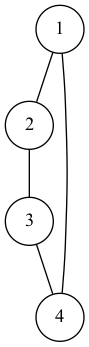
\includegraphics[height=10cm]{example1.png}
        \subcaption{辺操作前のグラフ}
        \label{fig:left}
    \end{minipage}
    \begin{minipage}{0.48\hsize}
        \centering
        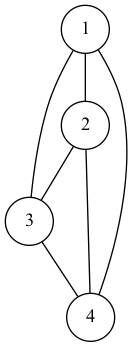
\includegraphics[height=10cm]{example1_.png}
        \subcaption{辺操作後のグラフ}
        \label{fig:right}
    \end{minipage}
    \caption{コストなしクラスター編集問題の問題例}
    \label{fig:left_right}
\end{figure}

$uv$を順序づけられていないペア${u,v} \in V$の省略形とする.
3頂点の組$uvw$について, $uv$と$vw$が辺であるが, $uw$が辺でない場合, 組$uvw$を$\textbf{衝突}$と呼ぶ.\\

\textbf{定理 1}[7]. グラフ$G$が$\textbf{クラスターグラフ}$であるための必要十分条件は, $G$に衝突が無いことである.\\

定理1より, コストなしクラスター編集問題の目標は, 辺操作を繰り返して衝突を全て削除することと言うこともできる.


\subsection{コストありクラスター編集問題}
コストなしクラスター編集問題はコスト関数$s$:$\binom{V}{2} \rightarrow \mathbb{Z}$を導入することで以下のように拡張できる.
頂点の部分集合$C \subseteq V$に属する任意の2頂点ペア$u,v$のコストが$s(uv) \ge 0$であるとき, $C$を$G$の$\textbf{クリーク}$と言う.
グラフ$(V,\{uv \in \binom{V}{2} | s(uv) > 0 \})$の各連結成分がクリークであるとき, $V$と$s$の組$(V,s)$を$\textbf{クラスターグラフ}$と呼ぶ.
頂点ペア$uv$のコスト$s(uv)$の符号を反転する操作を$\textbf{uvに対する辺操作}$と呼ぶ. この辺操作のコストは$|s(uv)|$と定義される.
また, 3頂点の組$uvw$について, $s(uv) > 0$, $s(vw) > 0$であるが, $s(uw) < 0$である場合, 組$uvw$を$\textbf{衝突}$と呼ぶ.
コストが正である頂点ペアのことを\textbf{正ペア}, コストが負である頂点ペアのことを\textbf{負ペア}と呼ぶ.\par
以上より, コストありクラスター編集問題は以下のように書ける.\\

\begin{screen}
    $\textbf{コストありクラスター編集問題}$ \\
    入力: \\
    \hspace{15pt} ・頂点集合$V$ \\*
    \hspace{15pt} ・コスト関数$s: \binom{V}{2} \rightarrow \mathbb{Z} $\\
    出力: \\
    \hspace{15pt} $(V,s)$をクラスターグラフに変形するために辺操作を行う頂点ペアの集合\\
    評価: \\
    \hspace{15pt} 辺操作のコストの和の最小化
\end{screen}

図2(a)にコストありクラスター編集問題の問題例を示す.
この例では, $s(2,3) = 5$, $s(2,4)=-5$となっており, 他の辺と比べて比較的大きな絶対値をもつ.
よって, 辺操作のコストを小さくするためにはこれらの編集を避ける必要がある.
頂点ペア$(1,3)$, $(1,4)$, $(3,4)$に辺操作を行った状態が図2(b)である.
このとき, 頂点集合$\{1,2,3\}$, $\{4\}$はクリークであり, $(V,s)$はクラスターグラフである.
この辺操作によって生じたコストは3である.

% 図の挿入
\begin{figure}[H]
    \centering
    \begin{minipage}{0.48\hsize}
        \centering
        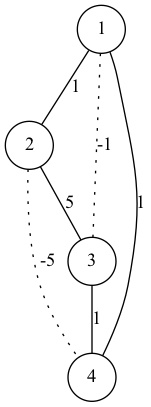
\includegraphics[height=10cm]{example2.png}
        \subcaption{辺操作前のコスト関数}
        \label{fig:left}
    \end{minipage}
    \begin{minipage}{0.48\hsize}
        \centering
        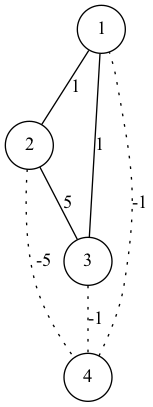
\includegraphics[height=10cm]{example2_.png}
        \subcaption{辺操作後のコスト関数}
        \label{fig:right}
    \end{minipage}
    \caption{コストありクラスター編集問題の問題例}
    \label{fig:left_right}
\end{figure}

コストなしクラスター編集問題は, コストありクラスター編集問題の全ての頂点ペア$uv$について, 辺コストが$s(uv) \in \{\pm 1\}$となっている場合にあたる.
頂点$u$, $v$間に辺が存在するとき$s(uv)=1$, 辺が存在しないとき$s(uv)=-1$という対応関係になっている.\par
また, パラメータ$k$を導入した問題についても, 説明する. 通常, 問題を解く上でパラメータは必須ではないが, クラスター編集問題は固定パラメータ容易であり, 本研究で用いる分枝限定アルゴリズムは固定パラメータ・アルゴリズムである.
したがって, 辺操作のコストを$k$とする問題を考える.

\begin{screen}
    $\textbf{パラメータ・コストありクラスター編集問題}$ \\
    入力: \\
    \hspace{15pt} ・頂点集合$V$ \\*
    \hspace{15pt} ・コスト関数$s: \binom{V}{2} \rightarrow \mathbb{Z} $\\
    \hspace{15pt} ・パラメータ$k \in \mathbb{Z}$ \\
    出力: \\
    \hspace{15pt} $(i)$ $(V,s)$をクラスターグラフにするコストが$k$以下の辺操作集合が存在するならば\\
    \hspace{15pt} \hspace{15pt}最小コスト辺操作集合を出力する. \\
    \hspace{15pt} $(ii)$それ以外の場合, 「解なし」を出力する
\end{screen}


\subsection{クラスター編集問題における整数計画問題と線形計画緩和}
本節では, コストありクラスター編集問題の整数計画問題としての表現と, 線形計画緩和について説明する.
$x$を0,1の2値をとるベクトルとする. 全ての頂点ペア$(i,j) \in \binom{V}{2}$に対して, $x_{ij}=0$ならば
$i$と$j$は同じクラスターに属し, $x_{ij}=1$ならば$i$と$j$は同じクラスターには属さないと対応させることで, クラスターグラフを$x$で表現する.
すると, 目的関数は$\sum_{(i,j \in \binom{V}{2}| s(ij) \ge 0)} s(ij) x_{ij} - \sum_{(i,j \in \binom{V}{2}| s(ij) < 0)} s(ij) (1-x_{ij}) $となる.
目的関数の前半部分は正ペアの辺を異なるクリークに分類するコスト, 後半部分は負ペアを同じクリークに分類するコストを表している.
制約は, 相異なる3頂点$i,j,k$に関して$x_{ij} \le x_{ik} + x_{jk}$を満たすこととする.
この制約を満たす$x$は, $V$の分割を表現する.
なぜなら, $x_{ij} > x_{ik} + x_{jk}$と仮定したとき$x_{ij}=1$, $x_{ik}=x_{jk}=0$となるが, このとき$i$と$k$は同じクラスターかつ$j$と$k$が同じクラスターであるが,
$i$と$j$が別のクラスターという矛盾が生じてしまうからである.\\
以上より, 整数計画問題の定式化は以下のとおりである.\\

\begin{mini*}
    {}{\sum_{(i,j \in \binom{V}{2}| s(i,j) \ge 0)}  s(ij) x_{ij} - \sum_{(i,j \in \binom{V}{2}| s(i,j) < 0)} s(ij) (1-x_{ij})}{}{}
    \addConstraint{x_{ij} \le x_{jk}+x_{ik} \quad \text{for all} \quad i,j,k \in V, \quad i \neq j \neq k \neq i}
    \addConstraint{x_{ij} \in \{0,1\} \quad \text{for all} \quad ij \in \binom{V}{2}.}
\end{mini*}

$x$を0,1の2値から$0 \le x \le 1$の実数へと緩和することにより, 線形計画問題(LP)が定義できる.\\
以上より, LPの定式は以下のとおりである.

\begin{mini*}
    {}{\sum_{(i,j \in \binom{V}{2}| s(i,j) \ge 0)}  s(ij) x_{ij} - \sum_{(i,j \in \binom{V}{2}| s(i,j) < 0)} s(ij) (1-x_{ij})}{}{}
    \addConstraint{x_{ij} \le x_{jk}+x_{ik} \quad \text{for all} \quad i,j,k \in V, \quad i \neq j \neq k \neq i}
    \addConstraint{0 \le x_{ij} \le 1 \quad \text{for all} \quad ij \in \binom{V}{2}.}
\end{mini*}


\section{禁止操作$\cdot$縮約操作}
本章では, パラメータ$\cdot$コストありクラスター編集問題について考える.
問題を解く上で, コスト$s(uv) \ge 0$であるような頂点ペア$uv$について, $\textbf{禁止}$あるいは$\textbf{縮約}$操作を行う場合がある.
以下ではこれらの操作について定義する.


\subsection{禁止操作}
$\textbf{禁止}$とはペア$uv$のコストを$-\infty$に設定することである.
禁止後のコストが$-\infty$なので, これ以降辺操作を$uv$に行うことができないことを意味している.
よって, $u$と$v$が同じクリークにならないことを強制する意味がある.\par
禁止操作によるコスト関数とパラメータの変化を定義する.
頂点集合$V$, コスト関数$s:\binom{V}{2} \rightarrow \mathbb{Z}$, パラメータ$k$である問題例$(V,s,k)$の頂点ペア$uv$を禁止操作した後の問題例を$(V,s',k')$と定義する.
このとき, $k'=k-s(uv)$, $s'$は$s'(uv)=-\infty$, $s'(u'v')=s(u'v')$ $(u'v' \in \binom{V}{2} \backslash \{uv\})$と定義する.
$uv$を禁止するときは, パラメータ$k$を$s(uv)$だけ減らす. これは, $uv$を禁止することは, $uv$に辺操作を行い, その後の操作を禁止することと同義であるからである.
禁止の例は図3に示した.\par
禁止操作後の問題例$(V,s',k')$にコスト$k'$以下の解があるとし, その解を$\mathbb{F'}$とする.
このとき, $\mathbb{F}=\mathbb{F'} \cup \{uv\}$と定義すると, $\mathbb{F}$のコストは$k$以下であり, 問題例$(V,s,k)$において$uv$に辺操作を行う解の中で最小コストのものとなる.
逆に$(V',s',k')$にコスト$k'$以下の解が存在しないならば, $(V,s,k)$においても$uv$に辺操作を行うコスト$k$以下の解は存在しない.

\begin{figure}[H]
    \centering
    \begin{minipage}{0.48\hsize}
        \centering
        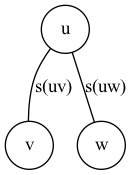
\includegraphics[height=5cm]{forbid.png}
        \subcaption{禁止前のグラフ}
        \label{fig:left}
    \end{minipage}
    \begin{minipage}{0.48\hsize}
        \centering
        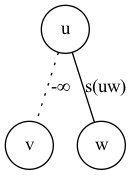
\includegraphics[height=5cm]{forbid_.png}
        \subcaption{$uv$を禁止後のグラフ}
        \label{fig:right}
    \end{minipage}
    \caption{禁止の実行例}
    \label{fig:left_right}
\end{figure}


\subsection{縮約操作}
$\textbf{縮約}$とは, 頂点$u$, $v$を単一の頂点$u'$に置き換え, 任意の頂点$w \in V \backslash \{u,v\}$について, 頂点ペア$uw$, $vw$を$u'w$に置き換える操作のことである.
この操作は$u$と$v$が同じクリークになることを強制する意味がある.
縮約操作による頂点集合, コスト関数とパラメータの変化を定義する.
頂点集合$V$, コスト関数$s:\binom{V}{2} \rightarrow \mathbb{Z}$, パラメータ$k$である問題例$(V,s,k)$の$uv$を縮約操作した後の問題例を$(V^*,s^*,k^*)$と書く.
縮約操作では, 頂点$u$と$v$を新たな頂点$u'$で置き換える.
つまり, $V^*=(V \cup \{u'\}) \backslash \{u,v\}$となる.
また, $k^*= k - \sum_{w \in V \backslash \{u,v\},s(uw)\cdot s(vw) < 0} \min\{|s(uw)|, |s(vw)|\}$, $s^*$は任意の$w \in V \backslash \{u,v\}$について
\[s^*(xw)=
\left\{
    \begin{array}{ll}
        s(uw)+s(vw) & {x=u'}\\
        s(xw) & {x \neq u'}\\
    \end{array}
    \right.
\]
と定義する.\par
縮約操作の例を図4に示す.
また, 負ペアを波線で表している.
図4では$s(uw)=2$, $s(vw)=-1$である.
この場合,縮約後のペア$u'w$コストは$s(uw)+s(vw)=1$となる.
このとき, パラメータは$\min\{|s(uw)|, |s(vw)|\}=|s(vw)|=1$だけ減る.\par
縮約操作後の問題例$(V^*,s^*,k^*)$がコスト$k^*$以下の解をもつとし, この解を$\mathbb{F^*}$とする.
$\overline{\mathbb{F}}$を, $\mathbb{F^*}$に含まれる頂点ペアのうち$u'$を含まないペアの集合とする.
また, $\mathbb{F}_u=\{u'w \in \mathbb{F^*} | w \in V^* \backslash \{u'\}\}$, $\mathbb{F'}_u= \{u'w \notin \mathbb{F^*} | w \in V^* \backslash \{u'\}\}$とする.
さらに$\overline{\mathbb{F}}_u = \{u''w | u'w \in \mathbb{F}_u, u'' \in \{u,v\}, s^*(u'w) \cdot s(u''w) < 0\}$, $\overline{\mathbb{F'}}_u = \{u''w | u'w \in \mathbb{F'}_u, u'' \in \{u,v\}, s^*(u'w) \cdot s(u''w) > 0\}$とする.
このとき, $f(\mathbb{F})= \overline{\mathbb{F}} \cup \overline{\mathbb{F}}_u \cup \overline{\mathbb{F'}}_u$と定義すると, $f(\mathbb{F})$のコストは$k$以下であり, 問題例$(V,s,k)$において$u$と$v$を同じクリークに分類する解の中で最小コストのものとなる.
逆に$(V^*,s^*,k^*)$にコスト$k^*$以下の解が存在しないならば, $(V,s,k)$においても$u$と$v$を同じクリークに分類するコスト$k$以下の解は存在しない.\par
$f(\mathbb{F})$の例を図5に示す.
図5(b)と図5(c)より$\mathbb{F^*}=\{u'w, wy\}$, $\overline{\mathbb{F}}=\{wy\}$, $\mathbb{F}_u=\{u'w\}$, $\mathbb{F'}_u=\{u'x\}$である.
また, 図5(a)より, $\overline{\mathbb{F}}_u=\{uw\}$, $\overline{\mathbb{F'}}_u=\{ux\}$である.
したがって, $f(\mathbb{F})= \overline{\mathbb{F}} \cup \overline{\mathbb{F}}_u \cup \overline{\mathbb{F'}}_u=\{uw, ux, wy\}$であり, 図5(a), 図5(d)からこれが解と一致することがわかる.
% 図の挿入

\begin{figure}[H]
    \centering
    \begin{minipage}{0.48\hsize}
        \centering
        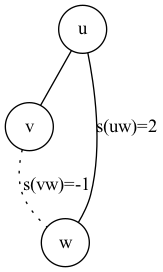
\includegraphics[height=5cm]{merge3.png}
        \subcaption{縮約前のグラフ}
        \label{fig:left}
    \end{minipage}
    \begin{minipage}{0.48\hsize}
        \centering
        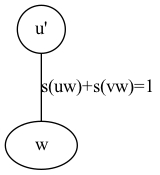
\includegraphics[height=5cm]{merge3_1.png}
        \subcaption{$uv$を縮約後のグラフ}
        \label{fig:right}
    \end{minipage}
    \caption{縮約の実行例($u'w$が正ペアの場合)}
    \label{fig:left_right}
\end{figure}


\begin{figure}[H]
    \centering
    \begin{minipage}{0.48\hsize}
        \centering
        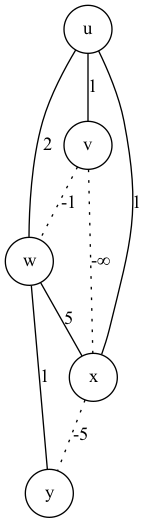
\includegraphics[height=7cm]{f01.png}
        \subcaption{縮約前のグラフ}
        \label{fig:left}
    \end{minipage}
    \begin{minipage}{0.48\hsize}
        \centering
        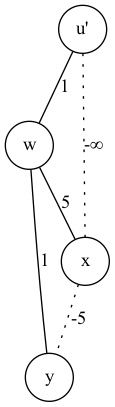
\includegraphics[height=7cm]{f02.png}
        \subcaption{$uv$を縮約後のグラフ}
        \label{fig:left-center}
    \end{minipage}
    \begin{minipage}{0.48\hsize}
        \centering
        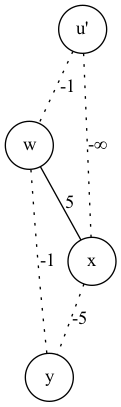
\includegraphics[height=7cm]{f03.png}
        \subcaption{$u'w$, $wy$を禁止後のグラフ}
        \label{fig:right-center}
    \end{minipage}
    \begin{minipage}{0.48\hsize}
        \centering
        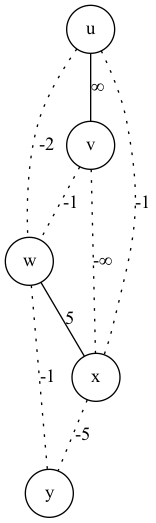
\includegraphics[height=7cm]{f04.png}
        \subcaption{クラスターグラフ}
        \label{fig:right}
    \end{minipage}
    \caption{$f(\mathbb{F})$の例}
    \label{fig:left_right}
\end{figure}

\clearpage


\section{アルゴリズム}
本研究では分枝限定法に基づくアルゴリズムについて検討する.
本章では5.1節で分枝限定法の全体像について説明し, その後, 詳細の説明を行う.


\subsection{分枝限定アルゴリズム}
本節では分枝限定アルゴリズムの説明を行う.
このアルゴリズムでは, 頂点集合$V$と頂点間のコスト$s:\binom{V}{2}\rightarrow\mathbb{Z}$が与えられる.
コスト$k$以下の辺操作集合が存在するならば最小コスト辺操作集合, コスト$k$以下の辺操作集合が存在しないならば「解なし」というメッセージを出力とする.
アルゴリズムはまず, グラフ内に衝突があるかを調べ, 存在すればその中から一つ選択する.
衝突が存在しなければ, そのグラフはクラスターグラフであるのでその時点で解を出力する.
組$uvw$を選択した衝突とし, 一般性を失うことなく$s(uv) > 0$とする.
アルゴリズムは$uv$を禁止して得られる問題例と, 縮約して得られる問題例をそれぞれ再帰的に解くことで, 元の問題を解く.

\begin{screen}
    $\textbf{分枝限定アルゴリズム}$ \\
    入力: \\
    \hspace{15pt} ・頂点集合$V$\\*
    \hspace{15pt} ・コスト関数$s:\binom{V}{2} \rightarrow \mathbb{Z}$\\
    出力: \\
    \hspace{15pt} ・頂点ペア集合もしくは「解なし」\\*
    $(1)$ $(V,s)$を入力として最適解の上界計算を行い, 出力された解のコストを$k$とする.\\
    $(2)$ $(V,s,k)$を入力として, 前処理を行う. 前処理の出力が「解なし」の場合は,\\
    \hspace{15pt}「解なし」を出力して終了. それ以外の場合は, 前処理の出力を$(\overline{V}, \overline{s}, \overline{k}, \overline{\mathbb{F}})$とする.\\
    $(3)$ 衝突が1つも無ければ$\overline{\mathbb{F}}$を出力して終了. $(\overline{V},\overline{s})$の衝突に含まれる正ペア$uv$を選択する.\\
    $(4)$ 問題例$(\overline{V}, \overline{s}, \overline{k})$で$uv$を禁止した問題例$(\overline{V},s',k')$を再帰的に解き, 得られた解を$\mathbb{F'}$とする.\\
    \hspace{15pt} $\mathbb{F'}$のコストを$s(\mathbb{F'})$とする. $\mathbb{F'}$が「解なし」ではない場合, $\overline{k}:=s(\mathbb{F})+s(uv)$とする.\\
    $(5)$ 問題例$(\overline{V}, \overline{s}, \overline{k})$で$uv$を縮約した問題例$(V^*,s^*,k^*)$を再帰的に解き, 得られた解を$\mathbb{F^*}$とする.\\
    $(6)$ $\mathbb{F^*}$が「解なし」ではない場合, $f(\mathbb{F^*}) \cup \overline{\mathbb{F}}$を出力する.\\
    \hspace{15pt}$\mathbb{F^*}$が「解なし」, $\mathbb{F'}$が「解なし」ではない場合, $\mathbb{F'}\cup \{uv\} \cup \overline{\mathbb{F}}$を出力する.\\
    \hspace{15pt}それ以外の場合, 「解なし」を出力する.
\end{screen}


\subsection{上界計算}
5.1節で与えた分枝限定アルゴリズムでは, ステップ$(1)$でパラメータ$k$を設定する.
このパラメータは, 最適解のコストの上界でなければアルゴリズムは解を出力しない.
よって, 解を計算するためには十分大きなパラメータを与える必要がある.
一方で, $k$が小さいほどアルゴリズムは不必要な探索を省略することができ, 計算時間の削減をすることができる.
よって, 本研究では, 分枝限定アルゴリズムを呼び出す前にヒューリスティックアルゴリズムで最適解のコストのなるべく小さな上界を求めることで高速化を目指す.
本研究で使用したヒューリスティックアルゴリズムは以下の3つである.\\
・ランダムピボット\\
・LPピボット\\
・LPを用いた分枝限定ヒューリスティック\\

\subsubsection{ランダムピボット}
$E$を正ペアからなる辺集合とし, 頂点集合$V$, 辺集合$E$からなる単純無向グラフを$G=(V,E)$で表す.
ランダムピボットは$G$内の1頂点をランダムに選ぶ.
選ばれた頂点を$v$とする.
頂点$v$に対して, $N(v)$をグラフ$G$における$v$の隣接頂点集合とする.
このとき, $v$自身は$N(v)$には含まれない.
また, $N[v]= N(v) \cup \{v\}$とする.
頂点集合$X \subseteq V$に対して, $N[X] = \bigcup_{v \in V} N[v]$とする. そして$N(X) = N[X] \backslash X$とする.
$N[v]$内の負ペアに辺操作を行うことで, クリークにする.
その後$N[v]$のカットに含まれる正ペアに辺操作を行うことで$N[v]$のみの連結成分ができる.
これを$(V,s)$がクラスターグラフになるまで反復する.\par
ランダムピボットの詳細は以下のとおりである.
\begin{screen}
    $\textbf{ランダムピボットアルゴリズム}$ \\
    入力: \\
    \hspace{15pt} ・頂点集合$V$\\*
    \hspace{15pt} ・コスト関数$s:\binom{V}{2} \rightarrow \mathbb{Z}$\\
    出力: \\
    \hspace{15pt} ・頂点ペア集合$\mathbb{F'}$\\*
    $(1)$ $V':=V$, $\mathbb{F'}:= \emptyset$とする.\\
    $(2)$ $|V'| > 1$を満たす限り, 以下の操作を繰り返し行う.\\
    \hspace{15pt} $(i)$ $V'$から頂点$v$を一様ランダムに選ぶ.\\
    \hspace{15pt} $(ii)$ $|N(v)| > 1$ならば$N(k)$内の任意の負ペア$ij$に対して, 辺操作を行う.\\
    \hspace{15pt} \hspace{15pt} これらの負ペアを$\mathbb{F'}$に追加する.\\
    \hspace{15pt} $(iii)$ $|N(v)|>0$ならば$N(v)$内の任意の頂点$x$と$V' \backslash N[v]$内の任意の頂点$y$からなる\\
    \hspace{15pt} \hspace{15pt} 正ペア$xy$について, 辺操作を行う. これらの正ペアを$\mathbb{F'}$に追加する. $V':=V \backslash N[v]$とする.\\
    $(3)$ $\mathbb{F'}$を出力する.
\end{screen}

\subsubsection{LPピボット}
LPピボットアルゴリズムは基本的にはランダムピボットアルゴリズムと同じだが, 違いは3.3節の線形計画問題(LP)の解を用いることである.
入力にLPの解$x:\binom{V}{2} \rightarrow [0,1]$を追加する.
LPピボットアルゴリズムの詳細は以下のとおりである.

\begin{screen}
    $\textbf{LPピボットアルゴリズム}$ \\
    入力: \\
    \hspace{15pt} ・頂点集合$V$\\*
    \hspace{15pt} ・コスト関数$s:\binom{V}{2} \rightarrow \mathbb{Z}$\\
    \hspace{15pt} ・LPの解$x: \binom{V}{2} \rightarrow [0,1]$\\
    出力: \\
    \hspace{15pt} ・頂点ペア集合$\mathbb{F'}$\\*
    $(1)$ $V':=V$, $\mathbb{F'} := \emptyset$とする.\\
    $(2)$ $|V'| > 1$を満たす限り, 以下の操作を繰り返し行う.\\
    \hspace{15pt} $(i)$ $V'$から頂点$v$を一様ランダムに選ぶ. $U := \emptyset$とする.\\
    \hspace{15pt} $(ii)$ $0 \le l \le 1$の範囲で有理数$l$を一様ランダムに選ぶ.\\
    \hspace{15pt} \hspace{15pt} そして, $l > x_{uv}$を満たす任意の頂点$u \in V'$を$U$に追加する.\\
    \hspace{15pt} $(iii)$ 両頂点が$U$に含まれる負ペアや片方が$U$, もう片方が$V \backslash U$に含まれる正ペアを$\mathbb{F'}$に追加する.\\
    \hspace{15pt} \hspace{15pt} $V':=V' \backslash U$とする.\\\
    $(3)$ $\mathbb{F'}$を出力する.
\end{screen}

\subsubsection{LPを用いた分枝限定ヒューリスティック}
LPを用いた分枝限定ヒューリスティックアルゴリズムはLPの解$x:\binom{V}{2} \rightarrow [0,1]$と衝突内の頂点ペア$uv$に関して, $x_{uv}=0$ならば縮約を行い, $x_{uv}=1$ならば禁止を行う.
その上で分枝限定アルゴリズムを適用し, 解を計算する.
LPの解の値が0,1以外の値が多ければ通常の分枝限定アルゴリズムとほとんど同じになってしまうことに注意が必要である.\par
以下がLPを用いた分枝限定ヒューリスティックアルゴリズムの詳細である.

\begin{screen}
    $\textbf{LPを用いた分枝限定ヒューリスティックアルゴリズム}$ \\
    入力: \\
    \hspace{15pt} ・頂点集合$V$\\*
    \hspace{15pt} ・コスト関数$s:\binom{V}{2} \rightarrow \mathbb{Z}$\\
    \hspace{15pt} ・LPの解$x:\binom{V}{2} \rightarrow [0,1]$\\
    出力: \\
    \hspace{15pt} ・頂点ペア集合もしくは「解なし」\\*
    $(1)$ $(V,s)$を入力として最適解の上界計算を行い, 出力された解の目的値を$k$とする.\\
    $(2)$ $(V,s,k)$を入力として, 前処理を行う. 前処理の出力が「解なし」の場合は,\\
    \hspace{15pt}「解なし」を出力して終了. それ以外の場合は, 前処理の出力を$(\overline{V}, \overline{s}, \overline{k}, \overline{\mathbb{F}})$とする.\\
    $(3)$ $(\overline{V},\overline{s})$の衝突$uvw$に含まれる正ペア$uv$を選択する. 衝突が1つも無ければ$\overline{\mathbb{F}}$を出力して終了.\\
    $(4)$ $x_{uv} = 1$ならば$(a)$を行う. $x_{uv}=0$ならば$(b)$を行う. それ以外は$(a)$,$(b)$両方行う.\\
    \hspace{15pt} $(a)$ $uv$を禁止した問題例$(V,s',k')$を再帰的に解き, 得られた解を$\mathbb{F'}$とする.\\
    \hspace{15pt} \hspace{15pt} $\mathbb{F'}$のコストを$s(\mathbb{F'})$とする. $\mathbb{F'}$が「解なし」ではない場合, $\overline{k}:=s(\mathbb{F})+s(uv)$とする.\\
    \hspace{15pt} $(b)$ 問題例$(\overline{V}, \overline{s}, \overline{k})$で$uv$を縮約した問題例$(V^*,s^*,k^*)$を再帰的に解き, 得られた解を$\mathbb{F'}$とする.\\
    $(5)$ $\mathbb{F^*}$が「解なし」ではない場合, $f(\mathbb{F^*}) \cup \overline{\mathbb{F}}$を出力する.\\
    \hspace{15pt}$\mathbb{F^*}$が「解なし」, $\mathbb{F'}$が「解なし」ではない場合, $\mathbb{F'}\cup \{uv\} \cup \overline{\mathbb{F}}$を出力する.\\
    \hspace{15pt}それ以外の場合, 「解なし」を出力する.
\end{screen}


\subsection{前処理}
前処理としてCaoとChen[11]が提案した辺カットに基づくカーネル化アルゴリズムを用いる.
カーネル化アルゴリズムは頂点集合$V$, コスト関数$s:\binom{V}{2} \rightarrow \mathbb{Z}$, パラメータ$k$を入力とする.
そして, アルゴリズムの操作によって変化した頂点集合$V'$, コスト関数$s':\binom{V}{2} \rightarrow \mathbb{Z}$, パラメータ$k'$, 辺操作を行った頂点ペアの集合$\mathbb{F}$を出力とする.
カーネル化アルゴリズム適用後は元の問題例と解が変わらないままサイズを小さくすることができるので, 計算の高速化に貢献する.\par
アルゴリズムに必要な定義を説明をする.
$E_s$を正ペアからなる辺の集合$\{uv \in \binom{V}{2} | s(uv) > 0 \}$とする.
また, 頂点集合$V$, 辺集合$E_s$からなる単純無向グラフを$G_s=(V,E_s)$で表す.
頂点集合$X \subset V$に対して, $\overline{X} = V \backslash X$と定義する.
2つの頂点部分集合$X$, $Y$に対して, 端点の一方が$X$に含まれて, もう一方が$Y$に含まれている辺集合を$E_s(X,Y)$とする.
このとき$E_s(X,\overline{X})$を$X$のカットと呼ぶ.
$X$のカットの合計コストを$\gamma(X)=\sum_{uv \in E_s(X,\overline{X})} s(uw)$とする.
$V$の頂点部分集合$X$に対して, $X$によって誘導される$G_s$の部分グラフを$G_s[X]$と書く.
$G_s[N[v]]$内のコストが負である頂点ペアの合計コストを$N[v]$の不足$\delta(v)$と呼ぶ.
つまり, $\delta(v) = \sum_{x,y \in N[v], \ s(xy) < 0} |s(xy)|$である.
これは$N[v]$をクリークにするためにかかるコストを表す.\par
カーネル化アルゴリズムは分枝限定アルゴリズムの前に行う.
元の問題の解を$\mathbb{F}$, カーネル化アルゴリズムと分枝限定アルゴリズムで得られた解をそれぞれ$\mathbb{F'}$, $\mathbb{F^*}$とすると, $\mathbb{F}=\mathbb{F'} \cup \mathbb{F^*}$である.
\begin{screen}
    $\textbf{カーネル化アルゴリズム}$ \\
    入力: \\
    \hspace{15pt} ・頂点集合$V$ \\*
    \hspace{15pt} ・コスト関数$s:\binom{V}{2} \rightarrow \mathbb{Z}$ \\
    \hspace{15pt} ・パラメータ$k\in\mathbb{Z}$\\
    出力: \\
    \hspace{15pt} ・頂点集合$\overline{V}$\\*
    \hspace{15pt} ・コスト関数$\overline{s}:\binom{\overline{V}}{2} \rightarrow \mathbb{Z}$\\
    \hspace{15pt} ・パラメータ$\overline{k}\in\mathbb{Z}$\\
    \hspace{15pt} ・頂点ペア集合$\overline{\mathbb{F}} \subseteq \binom{V}{2}$, もしくは「解なし」\\
    (1) $(\overline{V},\overline{s},\overline{k}) := (V,s,k), \quad \overline{\mathbb{F}} = \emptyset$とする.\\
    (2) $2\delta(v)+\gamma(N[v])<|N[v]|$を満たすような頂点$v \in \overline{V}$に対して, 以下の操作を行う.\\
    \hspace{15pt} $(i)$ $\overline{\mathbb{F}}$に$\overline{G}_{\overline{s}}[N[v]]$の全ての負ペアを追加する. これらのペアに辺操作を行いクリークにする.\\
    \hspace{15pt}\hspace{15pt} 発生したコストの分だけ$\overline{k}$を減少させる.\\
    \hspace{15pt}$(ii)$ 頂点集合$N(N[v])$の任意の頂点$x$について, $\overline{s}(\overline{E}(x,N[v])) \le \frac{|N[v]|}{2}$を満たすならば\\
    \hspace{15pt}\hspace{15pt} $\overline{E}_{\overline{s}}(x,N[v])$の正ペアを$\mathbb{\overline{F}}$に追加し, これらのペアに辺操作を行う.\\
    \hspace{15pt}\hspace{15pt} 発生したコストの分だけ$\overline{k}$を減少させる.\\
    \hspace{15pt}$(iii)$ $N(N[v])$に頂点が存在するなら$N[v]$を1頂点に縮約し,\\
    \hspace{15pt} \hspace{15pt} 発生したコストの分だけ$\overline{k}$を減少させる. 得られた問題例を$(\overline{V},\overline{s},\overline{k})$とする.\\
    (3) 上記の操作後, $\overline{k} < 0$ならば「解なし」を出力.\\
    \hspace{15pt} $\overline{k} \ge 0$ならば頂点集合$\overline{V}$, コスト関数$\overline{s}$,パラメータ$\overline{k}$と辺操作集合$\overline{\mathbb{F}}$を出力.
\end{screen}


\subsection{正ペア$uv$の選択}
本節では分枝限定アルゴリズムのステップ$(3)$で行う正ペア$uv$の選択方法について, いくつかのアルゴリズムを説明する.

\subsubsection{正ペア$uv$を選択する素朴なアルゴリズム}
衝突内の正ペア$uv$を選択する際の素朴なアルゴリズムは以下の通りである.

\begin{screen}
    \textbf{衝突内の正ペア$uv$を選択する素朴なアルゴリズム}\\
    入力: \\
    \hspace{15pt} ・頂点集合$V$ \\*
    \hspace{15pt} ・コスト関数$s:\binom{V}{2} \rightarrow \mathbb{Z}$ \\
    出力: \\
    \hspace{15pt} ・正ペアあるいは「解なし」\\*
    $(1)$ $\{u,v\} \in V$であるまだ未探索の正ペア$uv$を選ぶ.\\
    $(2)$ ある頂点$w \in V \backslash \{u,v\}$について, $uvw$が衝突ならば$uv$を出力して終了.\\
    $(3)$ まだ未探索の正ペアが存在するならば(1)に戻る. $uv$が存在しないならば「解なし」と出力して終了.
\end{screen}

頂点数を$n$とすると, 正ペア$uv$を選ぶを選ぶ計算量が$O(n^2)$, $uv$が衝突に含まれるかどうかを判定する計算量が$O(n)$である.
したがって, このアルゴリズムの計算量は$O(n^3)$である.

\subsubsection{衝突の数を考慮した選択}
次に頂点ペア$uv$を含む衝突の数が最大の正ペアを選択するアルゴリズムを与える.
$uv$が多くの衝突に含まれているほど一回の禁止, 縮約操作で多くの衝突をなくすことができ, 分枝限定アルゴリズムの計算効率が上がるからである.\par
\begin{screen}
    \textbf{衝突の数を考慮した正ペア$uv$の選択アルゴリズム}\\
    入力: \\
    \hspace{15pt} ・頂点集合$V$ \\*
    \hspace{15pt} ・コスト関数$s:\binom{V}{2} \rightarrow \mathbb{Z}$ \\
    出力: \\
    \hspace{15pt} ・正ペアあるいは「解なし」\\*
    $(1)$ $\{u,v\} \in V$である任意の正ペア$uv$を選ぶ.\\
    \hspace{15pt} $(a)$ $P_{uv}:=0$と設定する.\\
    \hspace{15pt} $(b)$ ある頂点$w \in V \backslash \{u,v\}$について, $uvw$ば衝突ならば, $P_{uv}:=P_{uv}+1$と更新する.\\
    $(2)$ $P_{uv} > 0$となる正ペア$uv$が存在しないならば, 「解なし」を出力する.\\
    \hspace{15pt}$P_{uv} > 0$となる正ペア$uv$が存在するならば, $P_{uv}$が最も大きい$uv$を出力する.
\end{screen}
計算量は5.4.1節で与えたアルゴリズムと同様に$O(n^3)$である.

\subsubsection{衝突の数を考慮した選択の簡略化}
5.1章で与えた分枝限定アルゴリズムでは再帰計算の度に正ペアの選択のための計算を行う.
1回の計算ではそれほど負担にはならないが, 再帰回数が大きくなるにつれて衝突の計算時間も無視できなくなる.
そこで再帰ごとに計算するのではなく再帰の深さに応じて計算を行うようにする.
具体的には, 衝突を求める際にその時点でグラフがもつ衝突を全て記憶しておく.
次に衝突を計算するまでは記憶した衝突を用いて再帰計算を行う.
前回計算した衝突が禁止, 縮約操作を行うことにより衝突でなくなる可能性があることに注意が必要である.
もし記憶した衝突がなければ, その時点で衝突の計算を行う.
図8に再帰の深さが3の倍数のときの例を示す.
この例では, 根(ノード1)で衝突計算を行い, 葉(ノード4,5,7,8,11,12,14,15)で再び衝突計算を行なっている.
実験では, 再帰の深さが5の倍数のときに衝突の再計算を行なっている.

\begin{figure}[H]
    \begin{center}
    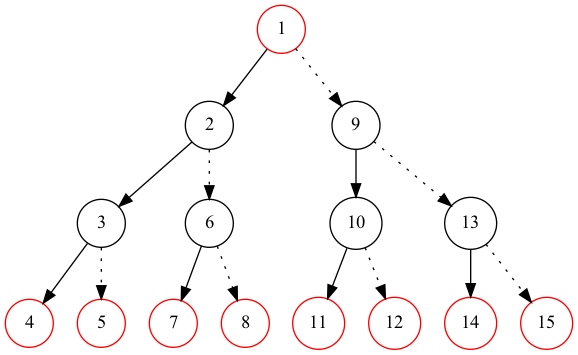
\includegraphics[width=10cm]{tree.png}
    \caption{再帰の深さが3の倍数のときに衝突計算を行う例(赤いノードで衝突を計算している)}
\end{center}
\end{figure}

\subsection{LPの解に応じて再帰中の禁止と縮約の順番を変える}
5.1節の分枝限定アルゴリズムではどの衝突も禁止, 縮約の順番で再帰計算を行なっていた.
そこでLPの解に応じて禁止と縮約の順番を入れ替えることにする.
LPの解$x:\binom{V}{2} \rightarrow [0,1]$と分資源的アルゴリズムのステップ3で選択された正ペア$uv$に対して, $x_{uv}=0$ならば順番を入れ替え縮約, 禁止の順に再帰計算を行う.
それ以外は通常通り禁止, 縮約の順で再帰計算を行う.
このアイデアは$x_{uv}=0$ (LPの解では$uv$は同じクラスター)ならば最適解でも$uv$は同じクラスターにいる可能性が高く,
$x_{uv}=1$ (LPの解では$uv$は別のクラスター)ならば最適解でも$uv$は別のクラスターにいる可能性が高いという仮定から生まれた.


\section{実験}
本研究では, 5章で提案したアルゴリズムを実装し, その性能を計算実験を通して評価して.
本章では, その結果について報告する.
\subsection{実験環境}
実装したアルゴリズムをいくつかの問題例に適用し, 結果を比較する.
データはクラスター編集問題を扱ったコンペティション, PACE Challenge 2021[26]で用いられた公開インスタンスの一部を用いる.
これらのインスタンスはすべてコストなし問題のインスタンスとなっており, 無向グラフによって表現されている.
プログラムを適用する際は, 3.2節で述べたようにコスト関数$s: \rightarrow \{0,1\}$を導入するすることで, コストあり問題として扱う.
プログラムの実行環境は表1, 使用したインスタンスの情報は表2で示している.
また, いくつかのアルゴリズムの中ではLPを解く必要がある.
LPを解く際は商用ソルバーであるILOG CPLEX[22]バージョン20.1を使用した.

\begin{table}[H]
    \begin{center}
        \caption{実行環境}
        \begin{tabular}{c|c}
    CPU         & 2.7GHz クアッドコアIntel Core i7 \\
    メモリ & 16GB 2133MHz LPDDR3 \\
    使用言語 & c++ \\
    時間の計測法 & c++のtimeモジュール \\
        \end{tabular}{}
    \end{center}
\end{table}

\begin{table}[H]
    \caption{インスタンスの情報}
    \label{table:data_type}
    \centering
    \begin{tabular}{l|ccr}
        \hline
        インスタンス名  & 頂点数  &  辺数 & 最適値  \\
        \hline \hline
        exact001  & 10  & 11  & 3\\
        exact003  & 20   & 73 & 42\\
        exact005  & 20  & 97 & 46\\
        exact007  & 30  &  147  & 86\\
        exact009  & 30 & 175  & 90\\
        exact011  & 30 & 291  & 81\\
        exact013  & 40 & 297  & 181\\
        exact015  & 40 & 360  & 164\\
        exact017  & 50 & 385  & 236\\
        exact019  & 50 & 489  & 298\\
        \hline
    \end{tabular}
\end{table}


\subsection{前処理の評価}
5.3節で与えた前処理がどれだけ問題サイズの削減に貢献できるか実験した.
exact001では3, exact005では1だけパラメータ$k$を削減できたが, 残りのインスタンスでは削減することができなかった.
カーネル化アルゴリズム適用後のグラフの頂点数は$O(2k)$となることが証明されているが, 使用したインスタンス元々は最適解に対して頂点数が比較的少ないので有意な効果が得られなかったと考えられる.


\subsection{上界計算アルゴリズム}
5.2節で述べた, ランダムピボット, LPピボット, LPを用いたヒューリスティックアルゴリズムを解の質と計算速度の観点から比較する.
具体的には, LPの解を用いたLPピボットがランダムピボットより優れているか, LPを用いた分枝限定ヒューリスティックが大きなグラフサイズでも短時間で解けるか, ランダムピボット, LPピボットに対して解がどれだけ優れているかといった点について議論する.\\
各アルゴリズムを適用した際の計算結果を表3, 表4に示す.
アルゴリズムを適用する際は, 制限時間を10分に設定し, 実行時間が制限時間を超えた場合はプログラムを打ち切った.
表では, 制限時間を超えた場合は"time out"と記載した. \par
表3は計算速度を比較した表である.
ランダムピボットとLPピボットはほとんど同じで無視できる差である.
LPを用いた分枝限定ヒューリスティックはexact011までは短時間で解けたが, exact013以降は制限時間以内に解くことができなかった.\par
表4は解の目的値を比較した表である.
ランダムピボットとLPピボットを見ると, exact005, exact011, exact015以外はランダムピボットが優れている.
LPを用いた分枝限定ヒューリスティックはランダムピボットとLPピボットに対して, 計算できたインスタンスでは全て優れた解を出力した.\par
LPピボットはランダムピボットに対して優れたアルゴリズムとは言えないが, 両者ともに高速なアルゴリズムなので, 両方計算し優れた解を用いることが効果的であると言える.
LPを用いた分枝限定ヒューリスティックは解の目的値は他の2つより優れているが, 計算時間が厳密アルゴリズムと大差ないことを考慮すると効果的なアルゴリズムであるとは言えない.
計算の簡略化など, 高速化のためのさらなる工夫が必要だと考えられる.

\begin{table}[H]
    \caption{ヒューリスティックアルゴリズムの計算時間[s]}
    \label{table:data_type}
    \centering
    \begin{tabular}{l|cccccccccr}
        \hline
        インスタンス名 & ランダムピボット  &  LPピボット & LPを用いた分枝限定ヒューリスティック\\
        \hline
        %\hline \hline
        exact001  & $4.3 \times 10^{-4}$   & $6.02 \times 10^{-4}$  & $1.53 \times 10^{-4}$ &\\
        exact003 & $1.667 \times 10^{-3}$  & $1.292 \times 10^{-3}$  & 0.317452\\
        exact005 & $1.055 \times 10^{-3}$ & $1.133 \times 10^{-3}$ & $5.651 \times 10^{-3}$ \\
        exact007 & $2.618 \times 10^{-3}$ & $2.422 \times 10^{-3}$ & 9.71585\\
        exact009 & $2.476 \times 10^{-3}$ & $2.427 \times 10^{-3}$ & 48.0892\\
        exact011 & $2.398 \times 10^{-3}$ & $5.266 \times 10^{-3}$ & $1.0851 \times 10^{-2}$\\
        exact013 & $5.672 \times 10^{-3}$  & $4.941 \times 10^{-3}$ & timeout\\
        exact015 & $4.907 \times 10^{-3}$ & $5.796 \times 10^{-3}$ & timeout\\
        exact017 & $8.43 \times 10^{-3}$ & $1.3271 \times 10^{-2}$ & timeout\\
        exact019 & $8.423 \times 10^{-3}$\ & $8.431 \times 10^{-3}$ & timeout\\
        \hline
    \end{tabular}
\end{table}

\begin{table}[H]
    \caption{ヒューリスティックアルゴリズムの出力解の目的値}
    \label{table:data_type}
    \centering
    \begin{tabular}{l|cccccccccr}
        \hline
        インスタンス名  & ランダムピボット  &  LPピボット & LPを用いた分枝限定ヒューリスティック\\
        \hline
        %\hline \hline
        exact001  & 3  & 3  & 3\\
        exact003 & 50 & 59 & 45\\
        exact005 & 55 & 46 & 46\\
        exact007 & 110 & 125 & 91\\
        exact009 & 116 & 140 & 100\\
        exact011 & 97 & 81 & 81\\
        exact013 & 219 & 251 & timeout\\
        exact015 & 206 & 165 & timeout\\
        exact017 & 316 & 343 & timeout\\
        exact019 & 388 & 424 & timeout\\
        \hline
    \end{tabular}
\end{table}


\subsection{上界計算アルゴリズムによる分枝限定アルゴリズムへの影響の比較}
分枝限定アルゴリズムにおいて, 5.2節で与えた上界計算のアルゴリズムで求めた上界をパラメータ$k$とする際の性能を評価する.
このために, 5.2節の3つのアルゴリズムで求めた上界の中で最良のものを$k$として分枝限定アルゴリズムを実行するプログラムと, $k$を1から順番に解が出力されるまで1ずつ増やしながら実行するプログラムを用意した.
以降, 前者をヒューリスティック, 後者をデフォルトと呼ぶ.
どちらも事前にカーネル化アルゴリズムでの前処理を行う.
両者を計算速度と再帰回数の観点から比較し, ヒューリスティックアルゴリズムでなるべく小さな上界を求めることがどれだけ有用かを評価する.\par
計算時間結果を表5に分枝限定アルゴリズムの再帰回数を表6に示す.
アルゴリズムを適用する際は, 制限時間を60分に設定し, 実行時間が制限時間を超えた場合はプログラムを打ち切った.
計算速度と再帰回数ともにヒューリスティックが圧倒的に優れていることがわかる.

\begin{table}[H]
    \caption{デフォルトとヒューリスティックの計算時間[s]}
    \label{table:data_type}
    \centering
    \begin{tabular}{l|cccccccccr}
        \hline
        インスタンス名  & デフォルト  &  ヒューリスティック\\
        \hline
        %\hline \hline
        exact001  & $2.26 \times 10^{-4}$  & $4 \times 10^{-6}$\\
        exact003 & 4.67355 & 0.872301\\
        exact005 & 9.47382 & 1.16827\\
        exact007 & 3234.17 & 540.535\\
        exact009 & 1652.6 & 347.233\\
        exact011 & 181.26 & 18.499\\
        exact013 & timeout & timeout\\
        exact015 & timeout & timeout\\
        exact017 & timeout & timeout\\
        exact019 & timeout & timeout\\
        \hline
    \end{tabular}
\end{table}

\begin{table}[H]
    \caption{デフォルトとヒューリスティックの再帰回数}
    \label{table:data_type}
    \centering
    \begin{tabular}{l|cccccccccr}
        \hline
        インスタンス名  & デフォルト  &  ヒューリスティック\\
        \hline
        %\hline \hline
        exact001  & 11  & 1\\
        exact003 & 116900 & 25637\\
        exact005 & 165694 & 23953\\
        exact007 & 43266710 & 7950997\\
        exact009 & 1628952 & 372877\\
        exact011 & 609277 & 76753\\
        exact013 & timeout & timeout\\
        exact015 & timeout & timeout\\
        exact017 & timeout & timeout\\
        exact019 & timeout & timeout\\
        \hline
    \end{tabular}
\end{table}


\subsection{再帰回数, 制限のための工夫の評価}
5.4節と5.5節で与えた再帰回数削減のための3つの手法を分枝限定アルゴリズムに導入した際の効果について検討する.
それぞれを単体および組み合わせて導入した場合の再帰回数と計算時間を比較していく.
それぞれの手法を提示した節に対応させて, それぞれ5.4.2, 5.4.3, 5.5と呼ぶことにする.
事前に前処理による問題サイズ削減, ヒューリスティックアルゴリズムを用いた最適値の上界計算は行なっている.\par
計算時間を表7に再帰回数を表8に示す.
アルゴリズムを適用する際は, 制限時間を60分に設定し, 実行時間が制限時間を超えた場合はプログラムを打ち切った.
単体で導入した場合の性能を比較すると, 5.4.2が一番優れていて, 5.4.3は単体だと逆効果になってしまうことがわかる.
複数の手法を組み合わせた場合を見ると, 5.4.2と5.4.3を組み合わせた手法が全ての場合の中で最も優れていた.
逆に, 5.5は単体だとそれなりの効果を発揮するが, 他の手法と組み合わせても良くなるどころかかえって悪化してしまった.

\begin{table}[H]
    \caption{再帰回数削減のための工夫を導入した際の計算時間[s]}
    \label{table:data_type}
    \centering
    \begin{tabular}{l|cccccccccr}
        \hline
        インスタンス名  & 工夫なし & 5.4.2  & 5.4.3 & 5.5 & 5.4.2+5.4.3  & 5.4.2+5.4.3+5.5\\
        \hline
        %\hline \hline
        exact001 & $4 \times 10^{-6}$ & $3 \times 10^{-6}$  & $6 \times 10^{-6}$ & $9 \times 10^{-6}$ & $10^{-6}$ & $10^{-5}$\\
        exact003 & 0.872301 & 0.81555 & 2.533869 & 1.05296 & 0.669425 & 1.09219\\
        exact005 & 1.16827 & 1.0278 & 1.04714 & 1.30373 & 0.717705 & 1.2961\\
        exact007 & 540.535 & 434.05 & timeout & 548.058 & 245.095 & 545.024\\
        exact009 & 347.233 & 172.684 & timeout & 199.822 & 78.8172 & 207.93\\
        exact011 & 18.499 & 15.7262 & 37.5391 & 17.4062 & 5.65564& 16.5961\\
        exact013 & timeout & timeout & timeout & timeout & timeout & timeout\\
        exact015 & timeout & timeout & timeout & timeout & timeout & timeout\\
        exact017 & timeout & timeout & timeout & timeout & timeout & timeout\\
        exact019 & timeout & timeout & timeout & timeout & timeout & timeout\\
        \hline
    \end{tabular}
\end{table}

\begin{table}[H]
    \caption{再帰回数削減のための工夫を導入した際の再帰回数}
    \label{table:data_type}
    \centering
    \begin{tabular}{l|cccccccccr}
        \hline
        インスタンス名  & 工夫なし & 5.4.2  & 5.4.3 & 5.5 & 5.4.2+5.4.3  & 5.4.2+5.4.3+5.5\\
        \hline
        %\hline \hline
        exact001 & 1 & 1 & 1 & 1 & 1\\
        exact003 & 25637 & 24657 & 252327 & 24999 & 51805 & 24999\\
        exact005 & 23953 & 20149 & 89277 & 20289 & 43129 & 20289\\
        exact007 & 7950997 & 6400075 & timeout & 6409683 & 11109719 & 6409683\\
        exact009 & 372877 & 1707615 & timeout & 1710295 & 2674653 & 1710295\\
        exact011 & 76753 & 63371 & 1354077 & 63411 & 96913 & 63411\\
        exact013 & timeout & timeout & timeout & timeout & timeout & timeout\\
        exact015 & timeout & timeout & timeout & timeout & timeout & timeout\\
        exact017 & timeout & timeout & timeout & timeout & timeout & timeout\\
        exact019 & timeout & timeout & timeout & timeout & timeout & timeout\\
        \hline
    \end{tabular}
\end{table}


\section{結論}
本研究では, 大規模なクラスター編集問題を解くための厳密アルゴリズムについて研究した.
基本となる分枝限定アルゴリズムにカーネル化アルゴリズムのアイデアを用いた前処理など高速化のために様々な工夫を導入し, 実際に実装し評価した.\par
導入した工夫の中では特にヒューリスティックで計算した最適解の上界をパラメータとして用いる手法は大きな効果を発揮した.
また, LPを用いた上界計算や再帰回数制限の工夫はともに期待した効果は発揮されなかった.\par
今後の展望としては, 分枝限定アルゴリズムの再帰中にヒューリスティックで最適解の上界を求め, 限定操作に用いる, より探索木のサイズが小さくなる分枝限定アルゴリズムの開発などが考えられる.
現状のアルゴリズムでは, 頂点数40以上の問題例を解くことが難しく, まだ実用的であるとは言い難い.
高速化のためのさらなる工夫が求められる.
\clearpage
\begin{thebibliography}{}
    \bibitem{} Bansal, N., Blum, A., Chawla, S.: Correlation clustering. Mach. Learn. 56(1),
    89--113 (2004)
    \bibitem{} Ben-Dor, A., Shamir, R., Yakhini, Z.: Clustering gene expression patterns. J.
    Comput. Biol. 6(3-4), 281--297 (1999)
    \bibitem{} Böcker, S., Briesemeister, S., Bui, Q.B.A., Truss, A.: Going weighted: Parameterized algorithms for cluster editing. Theor. Comput. Sci. 410(52), 5467--5480 (2009)
    \bibitem{} Böcker, S., Damaschke, P.: Even faster parameterized cluster deletion and cluster
    editing. Inform. Process. Lett. 111(14), 717--721 (2011)
    \bibitem{} Böcker, S., Briesemeister, S., Klau, G.W.: Exact algorithms for cluster editing:
    Evaluation and experiments. Algorithmica 60(2), 316--334 (2011)
    \bibitem{} Böcker, S.: A golden ratio parameterized algorithm for cluster editing. J. Discrete
    Algorithms 16, 79--89 (2012)
    \bibitem{} Böcker, S., Baumbach, J.: Cluster editing. In Paola Bonizzoni, Vasco Brattka, and
    Benedikt Löwe, editors, Proceedings of the 9th Conference on Computability in Europe, CiE 2013. LNCS, vol. 7921, pp. 33--44. (2013)
    \bibitem{} Bodlaender, H.L., Cai, L., Chen, J., Fellows, M.R., Telle, J.A., Marx, D.: Open problems in parameterized and exact computation. IWPEC 2006,
    Technical Report UU-Cs-2006-052, Department of Information and Computing Sciences. (2006)
    \bibitem{} Cao, Y., Chen, J.: Cluster editing: Kernelization based on edge cuts. Algorithmica
    64(1), 152--169 (2012)
    \bibitem{} Charikar, M., Guruswami, V., Wirth, A.: Clustering with qualitative information.
    J. Comput. System Sci. 71(3), 360--383 (2005)
    \bibitem{} Chen, J., Meng, J.: A 2k kernel for the cluster editing problem. J. Comput. Syst.
    Sci. 78(1), 211--220 (2012)
    \bibitem{} Delvaux, S., Horsten, L.: On best transitive approximations to simple graphs. Acta.
    Inform. 40(9), 637--655 (2004)
    \bibitem{} Downey, R.G., Fellows, M.R.: Parameterized Complexity. (1999)
    \bibitem{} Fellows, M.R.: The lost continent of polynomial time: Preprocessing and kernelization. In: Bodlaender, H.L., Langston, M.A. (eds.) IWPEC 2006. LNCS, vol. 4169,
    pp. 276--277. (2006)
    \bibitem{} Fellows, M.R., Langston, M.A., Rosamond, F.A., Shaw, P.: Efficient parameterized
    preprocessing for cluster editing. In: Csuhaj-Varjú, E., Ésik, Z. (eds.) FCT 2007.
    LNCS, vol. 4639, pp. 312--321. (2007)
    \bibitem{} Fomin, F.V., Kratsch, S., Pilipczuk, M., Pilipczuk, M., Villanger, Y.: Tight bounds
    for parameterized complexity of cluster editing. In: Proc. of Symposium on Theoretical Aspects of Computer Science (STACS 2013). LIPIcs, vol. 20, pp. 32--43.
    Schloss Dagstuhl-Leibniz-Zentrum fuer Informatik (2013)
    \bibitem{} Gramm, J., Guo, J., Hüffner, F., Niedermeier, R.: Automated generation of search
    tree algorithms for hard graph modification problems. Algorithmica 39(4), 321--347
    (2004)
    \bibitem{} Gramm, J., Guo, J., Hüffner, F., Niedermeier, R.: Graph-modeled data clustering:
    Fixed-parameter algorithms for clique generation. Theory Comput. Syst. 38(4),
    373--392 (2005)
    \bibitem{} Grötschel, M., Wakabayashi, Y.: A cutting plane algorithm for a clustering
    problem. Math. Program. 45, 52--96 (1989)
    \bibitem{} Guo, J.: A more effective linear kernelization for cluster editing. Theor. Comput.
    Sci. 410(8-10), 718--726 (2009)
    \bibitem{} Hartuv, E., Schmitt, A.O., Lange, J., Meier-Ewert, S., Lehrach, H., Shamir, R.:
    An algorithm for clustering cDNA fingerprints. Genomics 66(3), 249--256 (2000)
    \bibitem{} IBM ILOG CPLEX Optimization Studio. https://www.ibm.com/jp-ja/products/ilog-cplex-optimization-studio.
    \bibitem{} Křivánek, M., Moráve, J.: NP-hard problems in hierarchical-tree clustering. Acta
    Inform. 23(3), 311--323 (1986)
    \bibitem{}  Komusiewicz, C., Uhlmann, J.: Cluster editing with locally bounded modifications.
    Discrete Appl. Math. 160(15), 2259--2270 (2012)
    \bibitem{}  Mannaa, B.: Cluster editing problem for points on the real line: A polynomial time
    algorithm. Inform. Process. Lett. 110, 961--965 (2010)
    \bibitem{} PACE Challenge. https://pacechallenge.org/2021/.
    \bibitem{} Protti, F., da Silva, M.D., Szwarcfiter, J.L.: Applying modular decomposition
    to parameterized cluster editing problems. Theory Comput. Syst. 44(1), 91--104
    (2009)
    \bibitem{}  Rahmann, S., Wittkop, T., Baumbach, J., Martin, M., Truss, A., Böcker, S.: Exact
    and heuristic algorithms for weighted cluster editing. In: Proc. of Computational
    Systems Bioinformatics (CSB 2007), vol. 6, pp. 391--401 (2007)
    \bibitem{}  Shamir, R., Sharan, R., Tsur, D.: Cluster graph modification problems. Discrete
    Appl. Math. 144(1-2), 173--182 (2004)
    \bibitem{} Sharan, R., Maron-Katz, A., Shamir, R.: CLICK and EXPANDER: A system for
    clustering and visualizing gene expression data. Bioinformatics 19(14), 1787--1799
    (2003)
    \bibitem{} van Zuylen, A., Williamson, D.P.: Deterministic algorithms for rank aggregation and other ranking and clustering problems.
    In: Proceedings of Workshop on Approximation and Online Algorithms, WAOA 2007. LNSC, vol. 4927, pp. 260--273. (2008)
\end{thebibliography}
%\end{spacing}
\end{document}